\documentclass[tikz, border=20mm]{standalone}
\usepackage{amsmath,amssymb}
\usetikzlibrary{shadings}
\usepackage{xcolor}
\definecolor{tyell}{HTML}{FFFBAC}
\definecolor{tgray}{HTML}{332C39}
\definecolor{tblue}{HTML}{537FE7}
\definecolor{tred}{HTML}{E90064}
\definecolor{tnavy}{HTML}{301E67}
\begin{document}
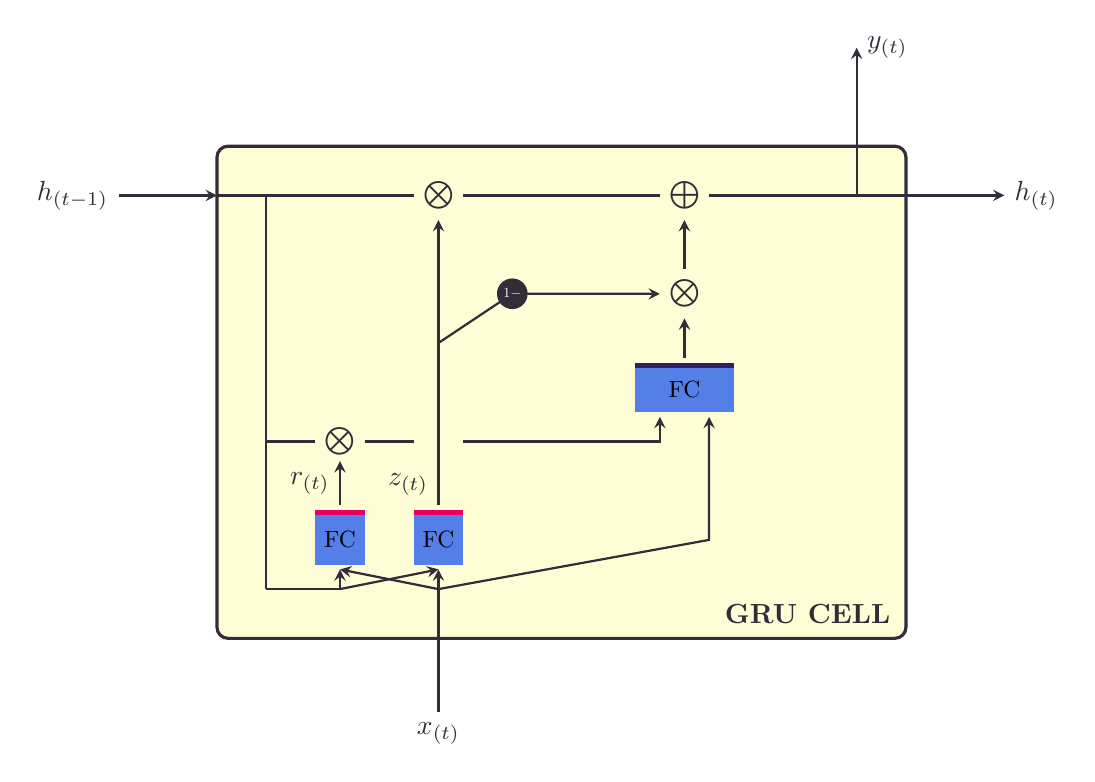
\begin{tikzpicture}[>=stealth, scale=1.25]
%The rectangle :
\filldraw[rounded corners, opacity=0.5, fill=tyell](0,0)rectangle(7,5);
\draw[rounded corners, line width=0.4mm, tgray] (0,0)rectangle(7,5);
%The connection lines and + x nodes : 
\draw[thick, tgray, ->] (-1,4.5)node[left] {$h_{(t-1)}$}--(0,4.5);
\draw[thick, tgray] (0,4.5)--(2,4.5);
\draw[thick, tgray] (2.5,4.5)--(4.5,4.5);
\draw[thick, tgray, ->] (5,4.5)--(8,4.5) node[right] {$h_{(t)}$};
\draw[thick, tgray, ->] (6.5,4.5)--(6.5,6) node[right] {$y_{(t)}$};
\node[tgray] (o1) at (2.25,4.5) {$\bigotimes$};
\node[tgray] (o2) at (4.75,4.5) {$\bigoplus$};
\draw[thick, tgray] (0.5,4.5)--(0.5,0.5);
\draw[thick, tgray] (0.5,2)--(1,2); 
\draw[thick, tgray] (1.5,2)--(2,2); 
\draw[thick, tgray, ->] (1.25,1.35)--(1.25,1.8) node[midway, left] {$r_{(t)}$};
\draw[thick, tgray, ->] (0.5,0.5)--(1.25,0.5)--(1.25,0.7);
\draw[thick, tgray, ->] (2.25,1.35)  node[above left] {$z_{(t)}$} --(2.25,4.25);
\draw[thick, tgray, ->] (2.25,-0.75) node[below] {$x_{(t)}$}--(2.25,0.7);
\draw[thick, tgray, ->] (2.5,2)--(4.5,2)--(4.5,2.25);
\draw[thick, tgray, ->] (1.25,0.5)--(2.25,0.7);
\draw[thick, tgray, ->] (2.25,0.5)--(1.25,0.7);
\node[tgray] (o3) at (1.25,2) {$\bigotimes$};
\coordinate(o) at (3,3.5);
\draw[tgray, thick] (2.25,3)--(o);
\draw[tgray, thick, ->] (o)--(4.5,3.5);
\filldraw[tgray] (o)circle(0.15) node[white, scale=0.5] {$1-$};
\draw[thick, tgray, ->] (4.75,2.85)--(4.75,3.25);
\draw[thick, tgray, ->]  (4.75,3.75)--(4.75,4.25);
\node[tgray] at (4.75,3.5) {$\bigotimes$};
\draw[thick, tgray, ->] (2.25,0.5)--(5,1)--(5,2.25);
%The small FC boxes
%Box 1
\fill[tblue] (1,0.75)rectangle(1.5,1.25); 
\node[scale=0.85] at (1.25,1) {FC};
\fill[tred] (1,1.25)rectangle(1.5,1.3);
%Box 2
\fill[tblue] (2,0.75)rectangle(2.5,1.25); 
\node[scale=0.85] at (2.25,1) {FC};
\fill[tred] (2,1.25)rectangle(2.5,1.3);
%Box 3
\fill[tblue] (4.25,2.3)rectangle(5.25,2.75);
\node[scale=0.85] at (4.75,2.525) {FC};
\fill[tnavy] (4.25,2.75)rectangle(5.25,2.8);
%GRU CELL
\node[tgray] at (6,0.25) {\textbf{GRU CELL}};
\end{tikzpicture}
\end{document}